\documentclass[a4paper, 11pt]{article}
\usepackage{geometry}
\usepackage{graphicx}
\usepackage{a4wide}
\usepackage{ulem}
\usepackage{amsthm}
\usepackage{amsmath}
\usepackage{amsfonts}
\usepackage{amssymb}
\usepackage[T1]{fontenc}
\usepackage{ngerman}
\usepackage{graphicx}
\usepackage{epic}
\usepackage{enumerate}
\usepackage{tabu}
\usepackage [latin1]{inputenc}
\geometry{a4paper,left=15mm,right=25mm,top=10mm,bottom=15mm}
%\renewcommand{\baselinestretch}{1.5}
\newcommand{\ol}{\overline}
\newcommand{\makeline}{\hrule\vspace{5pt}}
\newcommand{\ip}[2]{\left< #1, #2 \right>}

\title{5. �bungsblatt zu Software Qualit�t}
\author{Michel Meyer, Manuel Schwarz}

\begin{document}
  \maketitle

  \section*{Aufgabe 5.1}
  \subsection*{(a)}
  %\begin{figure}
		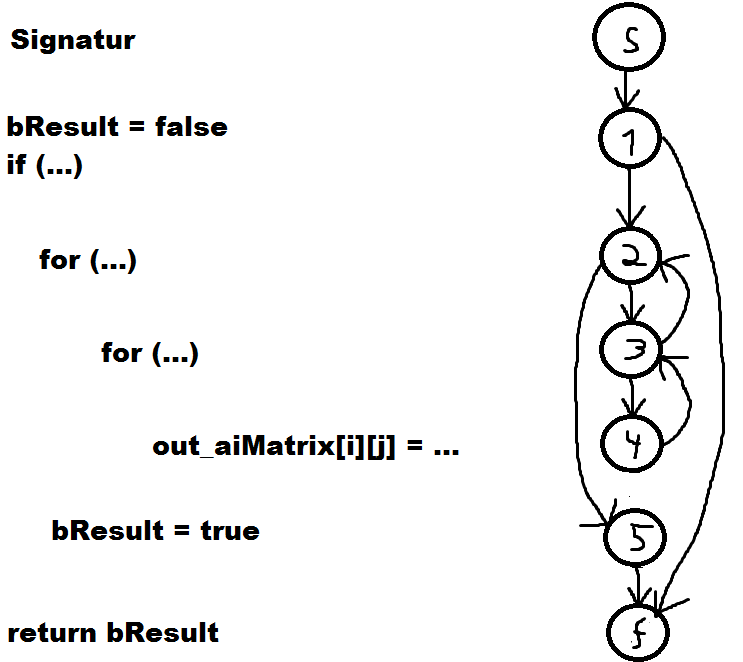
\includegraphics[width=\columnwidth]{Aufg1a.png}
	%\end{figure}
  

  \subsection*{(b)}
  \begin{tabular}[c]{|l|l|l|}\hline
  \textbf{Kategorie} & \textbf{ID} & \textbf{Pfad} \\\hline\hline
  Ohne     & A0 & $n_s, n_1, n_2, n_5, n_f$ \\\hline
  Schleife & B0 & $n_s, n_1, n_f$ \\\hline\hline
  Boundary & A1a& $n_s, n_1, n_2, n_3, n_4, n_3, n_2, n_5, n_f$ \\\hline
  Test     & A1b& $n_s, n_1, n_2, n_3, n_2, n_5, n_f$ \\\hline\hline
  Interior & A2c& $n_s, n_1, n_2, n_3, n_2, n_3, n_2, (n_3, (n_4, n_3)^k n_2)^m, n_5, n_f$ \\\hline
  Tests    & A2d& $n_s, n_1, n_2, n_3, n_2, n_3, n_4, n_3, n_2, (n_3, (n_4, n_3)^k n_2)^m, n_5, n_f$ \\\hline
           & A2e& $n_s, n_1, n_2, n_3, n_2, n_3, n_4, n_3, (n_4, n_3)^i, n_2, (n_3, (n_4, n_3)^k n_2)^m, n_5, n_f$ \\\hline
           & A3c& $n_s, n_1, n_2, n_3, n_4, n_3, n_2, n_3, n_2, (n_3, (n_4, n_3)^k n_2)^m, n_5, n_f$ \\\hline
           & A3d& $n_s, n_1, n_2, n_3, n_4, n_3, n_2, n_2, n_3, n_4, n_3, n_2, (n_3, (n_4, n_3)^k n_2)^m, n_5, n_f$ \\\hline
           & A3e& $n_s, n_1, n_2, n_3, n_4, n_3, n_2, n_3, n_4, n_3, (n_4, n_3)^i, n_2, (n_3, (n_4, n_3)^k n_2)^m, n_5, n_f$ \\\hline
           & A4c& $n_s, n_1, n_2, n_3, n_4, n_3, n_4, n_3, (n_4, n_3)^i, n_2, n_3, n_2, (n_3, (n_4, n_3)^k n_2)^m, n_5, n_f$ \\\hline
           & A4d& $n_s, n_1, n_2, n_3, n_4, n_3, n_4, n_4, (n_4, n_3)^i, n_2, n_2, n_3, n_4, n_3, n_2, (n_3, (n_4, n_3)^k n_2)^m, n_5, n_f$ \\\hline
           & A4e& $n_s, n_1, n_2, n_3, n_4, n_3, n_4, n_3, (n_4, n_3)^i, n_2, n_3, n_4, n_3, (n_4, n_3)^j, n_2, (n_3, (n_4, n_3)^k n_2)^m, n_5, n_f$ \\\hline
  \end{tabular}\\\\
  
	\noindent Erl�uterungen:\\
	\begin{tabular}[c]{|l|l|l|}\hline
	\textbf{ID} & \textbf{1. Schleifendurchlauf �u�ere Schleife} & \textbf{2. Schleifendurchlauf �u�ere Schleife} \\\hline\hline
	A2c         & 0x innere Schleife                             & 0x innere Schleife                             \\\hline
	A2d         & 0x innere Schleife                             & 1x innere Schleife                             \\\hline
	A2e         & 0x innere Schleife                             & mindestens 2x innere Schleife                  \\\hline
	A3c         & 1x innere Schleife                             & 0x innere Schleife                             \\\hline
	A3d         & 1x innere Schleife                             & 1x innere Schleife                             \\\hline
	A3e         & 1x innere Schleife                             & mindestens 2x innere Schleife                  \\\hline
	A4c         & mindestens 2x innere Schleife                  & 0x innere Schleife                             \\\hline
	A4d         & mindestens 2x innere Schleife                  & 1x innere Schleife                             \\\hline
	A4e         & mindestens 2x innere Schleife                  & mindestens 2x innere Schleife                  \\\hline
	\end{tabular}\\\\
	
	\noindent Hinter jeder Kombination steht der Term $(n_3, (n_4, n_3)^k n_2)^m$, damit nach den ersten beiden Schleifendurchl�ufen der �u�eren Schleife auch noch weitere Folgen k�nnen, deren innerer Ablauf beliebig ist.

\end{document}
